% !TeX program = lualatex
% !TeX encoding = utf8
% !TeX spellcheck = uk_UA
% !BIB program = biber
% !TeX root =../QChem.tex


\chapter{Наближені методи квантової механіки}

Лише невелика кількість задач квантової механіки можуть бути розв'язані математично точно. До таких задач відноситься, наприклад, задача про атом водню. Для систем, які складаються з багатьох частинок (атомів та молекул) точний розрахунок хвильової функції вже неможливий. Якщо відволіктись від проблем, які пов'язані з релятивістськими ефектами, то основна причина, яка не дає точно розв'язати рівняння Шредінґера полягає у взаємодії між електронами, саме наявність оператора міжелектронної взаємодії не дає можливості розділити змінні і отримати точний розв'язок.

Внаслідок цього практична придатність квантової механіки в значній мірі залежить від того, наскільки добре вдасться розробити наближені методи розрахунку хвильової функцій і фізичних величин. Однак, розробка наближених методів ні в якому разі не  обмежується лише завданням чисельно визначити фізичні або фізико-хімічні величини. Ці методи, крім цього, ще й повинні сприяти систематизації та інтерпретації емпіричних даних, розуміння основних закономірностей, формування нових модельних уявлень і розробці на їх основі загальних прогнозів.

Це стосується і прикладанню квантової механіки до проблем хімічного зв'язку і реакційної здатності --- тобто, до квантової хімії. Від результатів квантової хімії слід вимагати, щоб вони відповідали якісним правилам і уявленням про структуру і властивості молекул, які отримані з великого числа експериментальних даних. 

Якщо не враховувати рух ядра відносно центру мас, релятивістські ефекти, спін-спінову та спін-орбітальну взаємодію, то гамільтоніан багатоелектронного атому можна записати у вигляді (в атомних одиницях):
\begin{equation}\label{ManyAthomHamiltonian}
	\tcbhighmath{\hat{H} = \hat{T}_{e} + \hat{V}_{en} + \hat{V}_{ee} = -\frac12 \sum\limits_{i}^{N} \vect{\nabla}^2_i - \sum\limits_{i}^{N} \frac{Z}{r_i} + \frac12 \sum\limits_{i}^{N}\sum\limits_{\substack{j,\, j \neq i}}^{N}\frac{1}{r_{ij}},}
\end{equation}
де $\hat{T}_{e}$~--- кінетична енергія електрона, $\hat{V}_{en}$~--- потенціальна енергія взаємодії електрона та ядра, $\hat{V}_{ee}$~--- потенціальна енергія електрон-електронної взаємодії, $\vect{r}_i$~--- радіус-вектор, проведений від ядра до $i$-го електрона, $\vect{r}_{ij}$~--- радіус-вектор, що з'єднує положення $i$-го та $j$-го електронів. 

Рівняння Шредінґера з гамільтоніаном~\eqref{ManyAthomHamiltonian} має вигляд:
\begin{equation}\label{Shroedinger_equation}
		\hat{H} \psi(\vect{r}_1, \sigma_1; \vect{r}_2, \sigma_2; \ldots; \vect{r}_N, \sigma_N) = E\psi(\vect{r}_1, \sigma_1; \vect{r}_2, \sigma_2; \ldots; \vect{r}_N, \sigma_N).
\end{equation}

Точного розв'язку цього рівняння не існує. Основною причиною цього є останній доданок $\hat{V}_{ee} \propto r_{ij}^{-1}$, що описує електрон-електронну взаємодію. Саме його наявність не дозволяє розділити змінні в рівняння. Спроба врахувати цей доданок за допомогою теорії збурень призводить до поганих результатів, оскільки взаємодія між електронами має той же порядок, що і взаємодія електронів з ядром. Тому, особливого значення набувають наближені способи розв'язку рівняння Шредінґера. 

\section{Методи розв'язку рівняння Шредінґера}

\subsection{Метод теорії збурень}

Як було зазначено, теорія збурень призводить до незадовільних результатів при розв'язку рівняння Шредінґера для багатоелектронного атома, однак, якщо розв'язок буде отримано за допомогою інших наближених методів, то подальше уточнення можна проводити методами теорії збурень. Крім того для найпростішої багатоелектронної системи~--- атома гелію~--- цей метод дає задовільні результати, тому розглянемо даний метод.

Основна ідея теорії збурень полягає в тому, що всі взаємодії в системі можна умовно розділити на <<основні>> і <<збурення>>, а тому гамільтоніан системи можна представити у вигляді:
\begin{equation}\label{PerturbativeHamiltonian}
	\hat{H} = \hat{H}^0 + \hat{V},
\end{equation}
де  $\hat{H}^0$~--- <<незбурений>> гамільтоніан, для якого відомі власні функції і власні значення:
\begin{equation}\label{NonPerturbedEquation}
	\hat{H}^0\psi_n^{(0)} = E_n\psi_n^{(0)}.
\end{equation}
Функції $\{\psi_n^{(0)}\}$ фактично є спін-орбіталями, тому метод збурень природнім способом реалізує одноелектронне наближення. Доданок $\hat{V}$ в припущенні <<малості>> називається <<збуренням>>. В методі теорії збурень можна встановити математичний критерій <<малості>>, однак зрозуміло, що оператор можна вважати збуренням в тому випадку, якщо власні значення і власні функції рівняння Шредінґера
\begin{equation}
	\left( \hat{H}^0 + \hat{V}\right) \psi = E\psi
\end{equation}
мало відрізнятимуться від власних функцій і власних значень рівняння~\eqref{NonPerturbedEquation}.

В методі теорії збурень показується, що у першому наближенні теорії збурень енергія та хвильова функція мають вигляд:
\begin{align}\label{PerturbedValues}
	E_n &= E_n^{(0)} + \opbracket{\psi_n^{(0)}}{\hat{V}}{\psi_n^{(0)}},\\
	\psi_n &= \psi_n^{(0)} + \sum\limits_{\substack{m\\m \neq n}} \frac{\opbracket{\psi_n^{(0)}}{\hat{V}}{\psi_m^{(0)}}}{E_n^{(0)} - E_m^{(0)}} \psi_m^{(0)},
\end{align}
Очевидно, що критерієм <<малості>> збурення буде співвідношення:
\begin{equation}
	\left| V_{nm}\right|  \ll \left| E_n^{(0)} - E_m^{(0)} \right|.
\end{equation}



\begin{Example}[Застосування методу теорії збурень для атома гелію]
У випадку атома гелію, гамільтоніан~\eqref{ManyAthomHamiltonian} можна представити у вигляді:
\begin{equation}\label{HeliumAthomHamiltonian}
	\hat{H} = -\frac12 \vect{\nabla}^2_1  -\frac12 \vect{\nabla}^2_2 - \frac{Z}{r_2} - \frac{Z}{r_1} + \frac{1}{r_{12}}.
\end{equation}

Доданок, який враховує електрон-електронну взаємодію будемо вважати збуренням
\begin{equation}
	\hat{V} = \frac{1}{r_{12}}
\end{equation}
для основної задачі з гамільтоніаном:
\begin{equation}\label{HeliumAthomHamiltonian}
	\hat{H}^0 = -\frac12 \vect{\nabla}^2_1  -\frac12 \vect{\nabla}^2_2 - \frac{Z}{r_2} - \frac{Z}{r_1}.
\end{equation}

Основна задача легко розв'язується завдяки тому, що її можна легко розділити на дві незалежні задачі руху електрона у воднеподібному атомі з зарядом ядра $Z = 2$. Розв'язки цієї задачі добре відомі, зокрема для основного стану парагелію $1s$-орбіталь має вигляд:
\begin{equation}
	 (1s) = \frac{Z^{3/2}}{\sqrt\pi}e^{-Zr_i}.
\end{equation}

\begin{wrapfigure}[12]{O}[0pt]{5cm}
\begin{center}
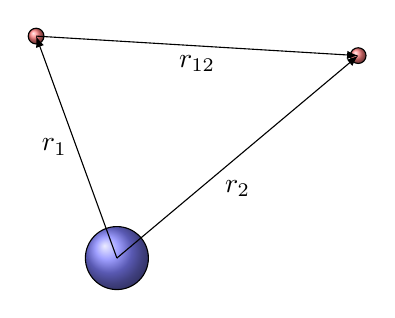
\begin{tikzpicture}
	\draw[ball color=blue!50] (0,0) circle (0.4);
	\draw[ball color=red!50]  (110:3) coordinate (E1) circle (0.1);
	\draw[ball color=red!50]  (40:4)  coordinate (E2) circle (0.1);
	
	\draw[-latex] (0,0) -- node[left] {$\vect{r}_1$} (E1);
	\draw[-latex] (0,0) -- node[below=5pt] {$\vect{r}_2$} (E2);
	\draw[-latex] (E1) -- node[below] {$\vect{r}_{12}$} (E2);
\end{tikzpicture}
\captionof{figure}{Схематичне зображення атома \ce{He}}
\end{center}
\end{wrapfigure}
Обидва електрони парагелію можна описувати однаковою хвильовою функцією, оскільки її спіни є протилежними і вони займають одну орбіталь. Загальна незбурена хвильова функція (координатна частина) є просто добутком $1s$-орбіталей координатну частину~\eqref{ground_state_parahelium}:
\begin{equation}\label{He_orbutal}
	\chi_0(\vect{r}_1, \vect{r}_2) = (1s)_1(1s)_2 = \frac{Z^{3}}{\sqrt\pi}e^{-Z(r_1 + r_2)}.
\end{equation}

Енергія відповідного основного стану являє собою суму енергій двох воднеподібних атомів:
\begin{equation}
	E_0 = -Z^2.
\end{equation}

Першою поправкою до енергії в теорії збурень є інтеграл:
\begin{equation}
	\opbracket{\chi_0}{\hat{V}}{\chi_0} = J = \int\limits_{V_1}\int\limits_{V_2} \frac{|(1s_1)|^2 |(1s_2)|^2}{r_{12}},
\end{equation}
який називається \emph{кулонівським\/}. З~\eqref{He_orbutal} кулонівський інтеграл приймає вигляд 
\begin{equation}\label{Columb_integral}
	 J = \frac{Z^6}{\pi^2} \int\limits_{V_1}\int\limits_{V_2}\frac{1}{r_{12}} e^{-2Z(r_1 + r_2)} dV_1dV_2 = + \frac58 Z.
\end{equation}

Отже повна енергія атома \ce{He}:
\begin{equation}\label{E_He_perturb}
	E = E_0 + J =  -Z^2 + \frac58 Z.
\end{equation}

Для гелію $Z = 2$, а тому $E = - 4 + \frac54 = -2.75$~Ха. Експериментальне значення $-2.9037$~Ха. Як бачимо, хоча перше наближення теорії збурень не є точним, але воно дає розумну оцінку енергії, навіть якщо <<збурення>>, тобто кулонівське відштовхування між електронами, є однаковим за порядком величини з усіма іншими взаємодіями. Більш того, основний стан, прийнятий в теорії збурень, зазвичай якісно правильний: точна хвильова функція для \ce{He} буде близька до добутку двох $1s$-функцій.

Однак, прикрою обставиною першого наближення теорії збурень є не скільки завищене значення енергії основного стану, скільки порушення теореми віріалу, згідно якої має виконуватись рівність $\left\langle T\right\rangle  = - E $. Так, повна енергія розрахована за теорією збурень $\ E  = -2Z^2 +\frac58 Z$ і кінетична $\left\langle T \right\rangle   = Z^2$,  що не задовольняє цій теоремі $Z^2 \neq Z^2 -\frac{5}{16} Z$.
\end{Example}
%=========================================================
\begin{problem}
    Отримайте вираз для середньої кінетичної та середньої потенціально енергії електронів в атомі гелію.
\end{problem}

%=========================================================
\begin{problem}
    Отримайте значення~\eqref{Columb_integral} кулонівського інтегралу.
\end{problem}

\subsection{Одноелектронне (орбітальне) наближення}

\begin{wrapfigure}[14]{O}[0pt]{5cm}
\begin{center}
	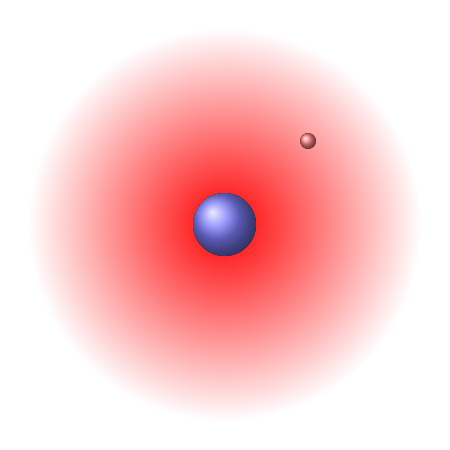
\begin{tikzpicture}
 		\path[inner color=red, outer color=white] (0,0) circle(2.5);
		\fill[ball color=blue!50] (0,0) circle (0.4);
		\fill[ball color=red!50]  (45:1.5) coordinate (E2) circle (0.1);
	\end{tikzpicture}
	\captionof{figure}{Ілюстрація одноелектронного наближення.}
	\label{pic:SCF_explanation}
\end{center}
\end{wrapfigure}
Основним наближенням, яке використовується в квантовій хімії є \emph{одноелектронне} наближення. В його основі лежить уявлення про існування індивідуальних станів кожного електрона, які являють собою стаціонарні стани руху електрона в деякому ефективному центральносиметричному полі, яке створюється ядром (або ядрами) і всіма іншими електронами (рис.~\ref{pic:SCF_explanation}). Іншими словами, у рамках такого наближення кожен електрон багатоелектронної системи є немов би незалежним. Для реалізації такого наближення останній доданок в гамільтоніані~\eqref{HeliumAthomHamiltonian} можна замінити на наближений:
\begin{equation}
	\frac12 \sum\limits_{i}^{N}\sum\limits_{\substack{j,\, j \neq i}}^{N}\frac{1}{r_{ij}} \approx \sum\limits_{i}^{N} \overline{V}(r_i),
\end{equation}
де потенціал $\overline{V}(r)$ може бути витлумачений як потенціал взаємодії електрона з розподіленим за об'ємом атома зарядом інших електронів. Важливо підкреслити, що взаємодія електрона залежить не від одночасного положення всіх інших електронів, а саме від їх усередненого положення. Потенціал $\overline{V}(r)$ також називають самоузгодженим, оскільки він залежить від стану атома, яке в свою чергу залежить від $\overline{V}(r)$. Тоді гамільтоніан системи можна представити у вигляді суми одночастинових гамільтоніанів, а отже, дає можливість розділити змінні. Цей гамільтоніан має вигляд:
\begin{equation}\label{approx_Hamiltonian}
	\hat{H}' = \sum\limits_{i}^{N}\hat{h}_i = -\frac12 \sum\limits_{i}^{N} \vect{\nabla}^2_i + \sum\limits_{i}^{N} \left( -\frac{Z}{r_i} + \overline{V}(r_i)\right).
\end{equation}


Таким чином, гамільтоніан \eqref{ManyAthomHamiltonian} $\hat{H}$ апроксимується гамільтоніаном \eqref {approx_Hamiltonian} $\hat{H}'$, а різницю $\hat{H}' - \hat{H} = W$ можна вважати збуренням і врахувати методом теорії збурень.

\subsection{Хвильова функція багатоелектронного атому}

Вигляд гамільтоніану \eqref{approx_Hamiltonian} дозволяє представити хвильову функцію у вигляді добутку, який має вигляд:
\begin{equation}\label{AtomPsiFunction}
	\psi(\vect{r}_1, \sigma_1; \vect{r}_2, \sigma_2; \ldots; \vect{r}_N, \sigma_N) = \psi_1 (\vect{r}_1, \sigma_1) \cdot \psi_2(\vect{r}_2, \sigma_2) \cdot\ldots \cdot \psi_N(\vect{r}_N, \sigma_N),
\end{equation}
де $\psi_i (\vect{r}_i, \sigma_i)$~--- власні хвильові функції оператора $\hat{h}_i$ і рівняння Шредінґера приймає вигляд системи рівнянь:
\begin{equation}
	 -\frac12 \vect{\nabla}^2_i \psi_i (\vect{r}_i, \sigma_i) +  \left( -\frac{Z}{r_i} + V(r_i)\right) \psi_i (\vect{r}_i, \sigma_i) = \epsilon_i \psi_i (\vect{r}_i, \sigma_i).
\end{equation}

У нерелятивістській квантовій теорії постулюється, що система частинок з напівцілими спінами, --- тобто, система ферміонів, до яких відносяться і електрони, --- має описуватися хвильовою функцією, яка змінює знак при перестановці координат і спінових змінних будь-якої пари електронів. Під перестановкою місцями розуміють <<обмін>> як просторовими, так і спіновими змінними будь-яких двох частинок. Тобто функція має бути \textit{антисиметричною} по відношенню до перестановки місцями двох довільних електронів, наприклад $i$-го і $j$-го:
\begin{multline}
	 \psi_A(\vect{r}_1, \sigma_1; \vect{r}_2, \sigma_2; \ldots; \vect{r}_i, \sigma_i; \ldots; \vect{r}_j, \sigma_j; \vect{r}_N, \sigma_N) = \\ = - \psi_A(\vect{r}_1, \sigma_1; \vect{r}_2, \sigma_2; \ldots; \vect{r}_j, \sigma_j; \ldots; \vect{r}_i, \sigma_i; \vect{r}_N, \sigma_N)
\end{multline}

Однак, хвильова функція~\eqref{AtomPsiFunction} не є симетричною, ані антисиметричною. Оскільки рівняння Шредінґера є лінійним, тому будь-яка лінійна комбінація його розв'язків також буде його розв'язком. Цей факт дає можливість побудувати антисиметричну функцію системи. Для цього треба взяти антисиметризовану лінійну комбінацію з $N!$ функцій, що утворені з кожної із $N!$ перестановок $N$ аргументів~\eqref{AtomPsiFunction}. 

Тому в якості своєї функції, що задовольняє принципу тотожності, слід взяти антисиметрична щодо перестановки частинок хвильову функцію, який називається \emph{детермінантом Слейтера}:


\begin{equation}\label{DetSlat}
\begin{gathered}
 \psi (\vect{r}_1, \sigma_1; \vect{r}_2, \sigma_2;\ldots;\vect{r}_N, \sigma_N)= \\ ={\frac {1}{\sqrt {N!}}}
 \left|
 {
 \begin{matrix}
 	\psi_{1}(\vect{r}_1, \sigma_1) & \psi_{1}(\vect{r}_2, \sigma_2) & \ldots & \psi_{1}(\vect{r}_i, \sigma_i) & \ldots & \psi_{1}(\vect{r}_N, \sigma_N) \\
 	\psi_{2}(\vect{r}_1, \sigma_1) & \psi_{2}(\vect{r}_2, \sigma_2) & \ldots & \psi_{2}(\vect{r}_i, \sigma_i) & \ldots & \psi_{2}(\vect{r}_N, \sigma_N) \\
 	\vdots                         & \vdots                         & \ddots & \vdots                         & \ddots & \vdots                         \\
 	\psi_{i}(\vect{r}_1, \sigma_1) & \psi_{i}(\vect{r}_2, \sigma_2) & \ldots & \psi_{i}(\vect{r}_i, \sigma_i) & \ldots & \psi_{i}(\vect{r}_N, \sigma_N) \\
 	\vdots                         & \vdots                         & \ddots & \vdots                         & \ddots & \vdots                         \\
 	\psi_{N}(\vect{r}_1, \sigma_1) & \psi_{N}(\vect{r}_2, \sigma_2) & \ldots & \psi_{N}(\vect{r}_i, \sigma_i) & \ldots & \psi_{N}(\vect{r}_N, \sigma_N)
 \end{matrix}
 }
 \right| 
\end{gathered}
\end{equation}

Детермінант Слейтера задає єдиний найпростіший спосіб побудови антисиметричної функції, що грунтується на одноелектронному наближенні, оскільки при перестановці двох стовпців (що відповідає перестановці двох електронів) детермінант, як відомо, змінює знак. З ~\eqref{DetSlat} також випливає, що якщо серед номерів станів виявляться два однакових (що відповідає рівності двох рядків), весь детермінант обертається в нуль. Таким чином, в одному і тому ж стані (тобто на одній і тій же спин-орбіталі) не може знаходитися більше одного електрона. Останнє твердження становить зміст \emph{принципу Паулі}, сформульованого в рамках одноелектронного наближення хвильової функції.

Одноелектронна функція називається називається \emph{спін-орбіталлю}:
\begin{equation}\label{spin-orbit}
	\psi_i(\vect{r}_i, \sigma_i),
\end{equation}
де $i$~--- номер електрона.


Оскільки гамільтоніан~\eqref{approx_Hamiltonian} не враховує спін-орбітальну взаємодію, то можливо розділити спінові і просторові змінні, тобто представити спін-орбіталь у вигляді добутку координатної та спінової функцій:
\begin{equation}
	\psi_i(\vect{r}_i, \sigma_i) = \chi_i(\vect{r}_i) \sigma_i.
\end{equation} 
Координатна функція $\chi_i(\vect{r}_i)$ називається \emph{орбіталлю}. Зрозуміло, що це пов'язано з класичним (планетарним) уявленням про атом як про сукупність електронів, що рухаються по власним орбітам. Одноелектронне наближення немов би дозволяє представити багатоелектронний атом з класичної точки зору, як сукупність електронів, однак в квантовій механіці поняття орбіти вже не існує навіть для одного електрона, тому одноелектронні стани називаються словом <<орбіталь>>, щоб дуже нагадувало слово <<орбіта>> і разом з тим відрізнялось від нього, а одноелектронне наближення називається також \emph{орбітальним}.

Для спінової функції прийнято позначення $\alpha$, якщо вона описує спін напрямлений вгору~$\uparrow$ і $\beta$~--- якщо спін напрямлений вниз~$\downarrow$:
\begin{equation}
	\sigma = 
		\begin{cases}
		\alpha, \, \uparrow \\
		\beta, \,  \downarrow
		\end{cases}.
\end{equation}

Розглянемо, яким чином багатоелектронна хвильова функція виражається через одноелектронні (тобто через спін-орбіталі) на прикладі атома \ce{He}.

\begin{Example}[Детермінанти Слейтера для атома гелію]
	Нарисуємо можливі розподіли електронів по $1s$- та $2s$-станам атома \ce{He}.
	\begin{center}
		\begin{tikzpicture}[
			upspinarrow/.pic = {\draw[-latex, blue] (0,-0.5) -- (0, 0.5);},
			downspinarrow/.pic = {\draw[latex-,red] (0,-0.5) -- (0, 0.5);}
					]
			\def\yshiftnode{-1.5}
			\def\xshiftnode{0.5}
			\def\distance{1.5}
			\draw[ultra thick]  (0,0) node[left] {$1s$} -- pic[pos=0.4] {upspinarrow}  pic[pos=0.6] {downspinarrow}+(1,0);
			\draw[ultra thick]  (0,\distance) node[left] {$2s$} -- +(1,0);
			\node at (\xshiftnode,\yshiftnode) {\itshape а)};
			\begin{scope}[xshift=2.5cm]
				\draw[ultra thick]  (0,0) -- pic {upspinarrow}  +(1,0);
				\draw[ultra thick]  (0,\distance) -- pic {upspinarrow} +(1,0);
				\node at (\xshiftnode,\yshiftnode) {\itshape б)};
			\end{scope}
			\begin{scope}[xshift=5cm]
				\draw[ultra thick]  (0,0) -- pic {downspinarrow}  +(1,0);
				\draw[ultra thick]  (0,\distance) -- pic {downspinarrow} +(1,0);
				\node at (\xshiftnode,\yshiftnode) {\itshape в)};
			\end{scope}
			\begin{scope}[xshift=7.5cm]
				\draw[ultra thick]  (0,0) -- pic {upspinarrow}  +(1,0);
				\draw[ultra thick]  (0,\distance) -- pic {downspinarrow} +(1,0);
				\node at (\xshiftnode,\yshiftnode) {\itshape г)};
			\end{scope}
			\begin{scope}[xshift=10cm]
				\draw[ultra thick]  (0,0) -- pic {downspinarrow}  +(1,0);
				\draw[ultra thick]  (0,\distance) -- pic {upspinarrow} +(1,0);
				\node at (\xshiftnode,\yshiftnode) {\itshape д)};
			\end{scope}
			\begin{scope}[xshift=12.5cm]
				\draw[ultra thick]  (0,0) -- +(1,0);
				\draw[ultra thick]  (0,\distance) -- pic[pos=0.4] {upspinarrow}  pic[pos=0.6] {downspinarrow} +(1,0);
				\node at (\xshiftnode,\yshiftnode) {\itshape е)};
			\end{scope}
		\end{tikzpicture}
\end{center}

Позначимо орбіталі атома гелію як $(1s)$ та $(2s)$. Конкретний аналітичний вигляд цих орбіталей поки не важливий. Вони наприклад можуть мати вигляд воднеподібних.

Детермінант Слейтера для випадку {\itshape а)\/} має вигляд:
\begin{equation}\label{ground_state_parahelium}
 \psi_0 ={\frac {1}{\sqrt {2}}}
 \left|
 {
 \begin{matrix}
 	(1s)_1\alpha_1 & (1s)_1\alpha_2 \\
 	(1s)_2\beta_1  & (1s)_2\beta_2
 \end{matrix}
 }
 \right| = {\frac {1}{\sqrt {2}}} (1s)_{1} (1s)_{2} (\alpha_1\beta_2 - \beta_1\alpha_2).
\end{equation}
Як видно, цей детермінант складається з добутку симетричної координатної частини $\chi_S = (1s)_1 (1s)_2$ та антисиметричної спінової частини $S_A^0 = (\alpha_1\beta_2 - \beta_1\alpha_2)$. Верхній індекс <<$0$>> показує, що повний спін системи дорівнює нулю. Отже, $\psi_0$-функцію можна записати як:
\begin{equation}\label{ground_state_parahelium_spin}
	\psi_0 = \chi_S S_A^0.
\end{equation}

Для випадку {\itshape б)\/}:
\begin{equation}
 \psi_1 ={\frac {1}{\sqrt {2}}}
 \left|
 {
 \begin{matrix}
 	(1s)_1\alpha_1 & (1s)_2\alpha_2 \\
 	(2s)_1\alpha_1  & (2s)_2\alpha_2
 \end{matrix}
 }
 \right| = {\frac {1}{\sqrt {2}}} \alpha_1 \alpha_2 ((1s)_1(2s)_2 -(2s)_1(1s)_2),
\end{equation}
$\psi_1$-функцію можна записати як:
\begin{equation}
	\psi_1 = \chi_A S_S^{+1},
\end{equation}
верхній індекс <<$+1$>> показує, що повний спін системи в цьому стані дорівнює $+1$.

Для випадку {\itshape в)\/}:
\begin{equation}
 \psi_2 = {\frac {1}{\sqrt {2}}}
 \left|
 {
 \begin{matrix}
 	(1s)_1\beta_1 & (1s)_2\beta_2 \\
 	(2s)_1\beta_1  & (2s)_2\beta_2
 \end{matrix}
 }
 \right| = {\frac {1}{\sqrt {2}}} \beta_1 \beta_2 ((1s)_1(2s)_2 -(2s)_1(1s)_2) = \chi_A S_S^{-1}
\end{equation}


Для випадків {\itshape г)\/} та {\itshape д)\/} не можна побудувати однодетермінантні функції, треба брати лінійні комбінації детермінантів. 

Так, для випадку {\itshape г)\/}:
\begin{equation}
	\psi_3 = {\frac {1}{\sqrt {2}}} = (\psi_5 + \psi_6) = \chi_A S_S^0,
\end{equation}
а  для випадку {\itshape д)\/}:
\begin{equation}
	\psi_4 = {\frac {1}{\sqrt {2}}} = (\psi_5 - \psi_6) = \chi_S S_A ^0 ,
\end{equation}
де
\begin{equation}
 \psi_5 = {\frac {1}{\sqrt {2}}}
 \left|
 {
 \begin{matrix}
 	(1s)_1\alpha_1 & (1s)_2\alpha_2 \\
 	(2s)_1\beta_1  & (2s)_2\beta_2
 \end{matrix}
 }
 \right|,
\end{equation}
\begin{equation}
 \psi_6 = {\frac {1}{\sqrt {2}}}
 \left|
 {
 \begin{matrix}
 	(1s)_1\beta_1 & (1s)_2\beta_2 \\
 	(2s)_1\alpha_1  & (2s)_2\alpha_2
 \end{matrix}
 }
 \right|.
\end{equation}

для випадку {\itshape е)\/} має вигляд:
\begin{equation}
 \psi_7 ={\frac {1}{\sqrt {2}}}
 \left|
 {
 \begin{matrix}
 	(2s)_1\alpha_1 & (2s)_1\alpha_2 \\
 	(2s)_2\beta_1  & (2s)_2\beta_2
 \end{matrix}
 }
 \right| = {\frac {1}{\sqrt {2}}} (2s)_{1} (2s)_{2} (\alpha_1\beta_2 - \beta_1\alpha_2).
\end{equation}
\end{Example}

Системи, в яких електрони займають орбіталі попарно, називаються системами з \emph{закритими (замкненими) електронними оболонками\/}. Для них детермінант Слейтера складається з двічі зайнятих електронами (з протилежними спинами) орбіталей, число яких дорівнює половині числа електронів. Системи, у яких електрони займають орбіталі по одинці (неспарені орбіталі) утворюють \emph{відкриті (незамкнені) оболонки}. Як правило, системи з непарним числом електронів в основному стані мають незамкнені зовнішні оболонки. 

Оболонки зображені на рисунках {\itshape а)\/} та {\itshape е)\/} є зманеними оболонками. Всі інші оболонки є незамкненими.

Як показує дослід, в спектрі газоподібного гелію є трикратно вироджені рівні~--- \emph{триплети}, та невироджені~--- \emph{синглети}. Атоми, які утворюють спектроскопічний триплет називаються \emph{ортогелієм}, а синглет~--- \emph{парагелієм}. 

Хвильові функції, які описують пара- та ортогелій можна розділити на дві групи:
\begin{itemize}
\item Перша група~--- хвильові функції, які містять три симетричні спінові функції $S_S^{+1}$, $S_0^0$ та $S_0^{-1}$:
\[
	\psi_1 = \chi_A S_S^{+1}, \psi_2 =  \chi_A S_S^{-1}, \psi_3 =  \chi_A S_S^0
\]
 Для таких функцій повне спінове число дорівнює $S = 1$, а його проекції приймають значення $M_S = +1, 0, -1$. Ця група утворює триплет.
\item Друга група~--- хвильова функція, яка містить антисиметричну спінову функцію $S_A^{0}$:
\[
	\psi_0 = \chi_S S_A ^0.
\]
Для цієї функції $S = 0$ і $M_S = 0$. Це синглет.
\end{itemize}

Функція $\psi_4$ описує збуджений стан парагелію, оскільки її спінова частина антисиметрична $S_A ^0$, а $\psi_4$~--- збуджений стан ортогелію, оскільки її спінова частина симетрична $S_S^0$.

Якщо нехтувати спін-орбітальною взаємодією, то переходи між орто- та парагелієм ними (з випромінюванням або поглинанням світла) заборонені через ортогональність спінових функцій. У зв'язку з цим ці стани є метастабільними (живуть місяці).


%=========================================================
\begin{problem}
    Побудуйте детермінант Слейтера для основного стану атомів 
	\begin{enumerate*}[label=\alph*)]
		\item \ce{Li},
		\item \ce{Be}.
	\end{enumerate*}	
%\begin{solution}
%	\begin{enumerate}[label=\alph*)]
%		\item \ce{Li}	
%			\begin{equation}
%				\psi_{\ce{Li}} = {\frac {1}{\sqrt {6}}}
%					 \left|
%					 {
%					 \begin{matrix}
%					 	(1s)_1\alpha_1 & (1s)_1\beta_1 & (2s_1)\alpha_1 \\
%					 	(1s)_2\alpha_2 & (1s)_2\beta_2 & (2s_2)\alpha_2 \\
%					 	(1s)_3\alpha_3 & (1s)_3\beta_3 & (2s_3)\alpha_3
%					 \end{matrix}
%					 }
%					 \right|.
%			\end{equation},
%		\item \ce{Be}
%			\begin{equation}
%				\psi_{\ce{Be}} = {\frac {1}{2\sqrt {6}}}
%					 \left|
%					 {
%					 \begin{matrix}
%					 	(1s)_1\alpha_1 & (1s)_2\alpha_2 & (1s)_3\alpha_3 & (1s)_4\alpha_4 \\
%					 	(1s)_1\beta_1  & (1s)_2\beta_2  & (1s)_3\beta_3  & (1s)_4\beta_4  \\
%					 	(2s)_1\alpha_1 & (2s)_2\alpha_2 & (2s_3)\alpha_3 & (2s_4)\alpha_4 \\
%					 	(2s)_1\beta_1  & (2s)_2\beta_2  & (2s_3)\beta_3  & (2s_4)\beta_4
%					 \end{matrix}
%					 }
%					 \right|.
%			\end{equation}	
%	\end{enumerate}
%\end{solution}
\end{problem}

%=========================================================
\begin{problem}
    Розгляньте випадок системи в якій число електронів більше числа орбіталей. Побудуйте для такої системи детермінінт Слейтера.
%\begin{solution}
%			\begin{equation}
%				\psi = {\frac {1}{\sqrt {6}}}
%					 \left|
%					 {
%					 \begin{matrix}
%					 	(1s)_1\alpha_1 & (1s)_2\alpha_2 & (1s_3)\alpha_3 \\
%					 	(1s)_1\beta_1  & (1s)_2\beta_2  & (1s_3)\beta_3  \\
%					 	(1s)_1\alpha_1 & (1s)_2\alpha_2 & (1s_3)\alpha_3
%					 \end{matrix}
%					 }
%					 \right|.
%			\end{equation}
%	У детермінанті перший рядок дорівнює третьому і тому цей визначник тотожно дорівнює нулю. Отже, число орбіталей в системі може, принаймні, дорівнювати числу електронів і тому в системі не може бути більше одного електрона з чотирма однаковими квантовими числами (принцип Паулі).
%\end{solution}
\end{problem}

\subsection{Варіаційні методи} 

Основна ідея методу полягає у використанні наближених, або <<пробних>> хвильових функцій.

В квантовій хімії зазвичай використовують два основних типа варіаційних методів:
\begin{enumerate}
\item У випадку системи багатьох частинок шукану хвильову функцію 
\end{enumerate}
В в якості <<пробної>> функції, що описує квантово-механічну систему, як правило можна вибрати таку, що залежить від ряду параметрів:
\begin{equation}\label{ArbFunction}
	\psi = \psi(a_1, a_2, \ldots, a_N),
\end{equation}
або як \textit{лінійну комбінацію деяких лінійно незалежних функцій} $\{\chi_i\}$, які називаються \emph{базисними} (метод Рітца):
\begin{equation}\label{Ritz}
	\psi = \sum\limits_{i}^N a_i \chi_i.
\end{equation} 
Параметри $a_i$ (в загальному випадку комплексні) в методі вважаються невідомими. Вибір же  базисних функцій ґрунтується на якісному аналізі можливих розв'язків задачі. Наприклад, для атомів це можуть бути воднеподібні хвильові функції.

Далі, згідно постулатів квантової механіки енергію системи в стані $\psi$ можна розрахувати як:
\begin{equation}\label{MedianEnergy}
	E  = \frac{\opbracket{\psi}{\hat{H}}{\psi}}{\bracket{\psi}{\psi}}.
\end{equation}
Як видно з цього виразу, значення енергії залежить від $\psi$-функції, тобто \emph{енергія є функціоналом}. 
\emph{Варіаційний метод стверджує, що найбільш наближеним значенням енергії до точного значення буде саме екстремальне (мінімальне) значення функціоналу.} 

Процедура знаходження мінімального значення полягає в наступному: для отримання параметрів $a_i$, які відповідають мінімальному значенню функціоналу енергії використовують відомі умови знаходження екстремуму:
\begin{equation}\label{ExtremumE}
	\frac{\partial E}{\partial a_i} = 0,
\end{equation}
які утворюють систему $N$ алгебраїчних рівнянь.

В методі Рітца  у виразі для $\psi$-функції~\eqref{Ritz} невідомими є саме параметри $a_i$, а базисні функції $\{\chi_i\}$ є цілком фіксованими, тому, виконуючи диференціювання в \eqref{ExtremumE}, отримаємо систему $N$ алгебраїчних рівнянь, яка має вигляд:
\begin{equation}
	\sum\limits_{j} (H_{ij} - ES_{ij})a_j = 0 
\end{equation}
де $H_{ij} = \opbracket{\chi_i}{\hat{H}}{\chi_j}$~--- матричні елементи гамільтоніана в базисі функцій $\{\chi_i\}$, а $S_{ij} = \bracket{\chi_i}{\chi_j}$~--- інтеграли перекривання.

Отримана система $N$ однорідних лінійних рівнянь дозволяє знайти параметри $a_i$, що забезпечують мінімум функціоналу~\eqref{MedianEnergy}. Щоб її розв'язати, необхідно прирівняти нулю визначник (детермінант), складений з коефіцієнтів при $a_i$:
\begin{equation}
	\mathrm{det}\left(H_{ij} - ES_{ij}\right) = 0.
\end{equation}

Важливо відмітити, що отримане таким чином мінімальне значення енергії є оцінкою зверху, тобто $E_{\min} \ge E_0$, де знак рівності буде лише у випадку точної $\psi$-функції  системи. На скільки розрахована енергія вища ніж точна з цього методу не відомо, сама ж його ефективність залежить від того, на скільки вдало вибрані пробні функції, що апроксимують точний розв'язок при знайдених параметрах $a_i$.

\begin{Attention}
	Універсального рецепту для вибору цих функцій та параметрів нема. В якості <<пробних>> функцій можна вибирати, наприклад,  власні функції гамільтоніана незбуреної задачі.
\end{Attention}

\begin{Attention}
	Точність значення енергії зазвичай набагато вище, ніж точність хвильової функції, для якої ця енергія визначається. Дійсно, енергія в в будь-якому квантовому стані є функціоналом вигляду \eqref{MedianEnergy}, і помилка в його визначенні квадратична щодо помилки хвильової функції. Таким чином, якщо відхилення хвильової функції від її точного виразу пропорційно малому параметру $\epsilon$, то значення енергії буде відрізнятися від точного на величину, пропорційну $\epsilon^2$, а це означає що  уточнення пробних функцій призводить до значно швидшого наближення величини $Е$ до точного значення, ніж самих пробних функцій.
\end{Attention} 

\begin{Example}[Застосування варіаційного методу для атома гелію]
В якості <<пробної>> функції ми візьмемо функції~\eqref{ground_state_parahelium} $\psi_0 = \chi_0 S_0^0$. Оскільки гамільтоніанн~\eqref{HeliumAthomHamiltonian} не містить спінових змінних, то для процедури варіювання обмежимось лише координатною частиною:
\begin{equation}\label{coordinate_ground_state_parahelium}
	\chi_0(\vect{r}_1, \vect{r}_2) = (1s)_1(1s)_2 = \frac{Z_e^{3}}{\sqrt\pi}e^{-Z_e(r_1 + r_2)},
\end{equation}
однак пам'ятаємо, що повна $\Psi$~--- функція є добутком спінової, координатної частин та фазового множника $e^{-\frac{E}{\hbar} t}$.

Невідомим параметром, по якому ми будемо варіювати енергію, зручно вибрати заряд ядра $Z_e$. Такий, з першого погляду дивний вчинок, грунтується на інтуїтивно зрозумілій ідеї \emph{екранування} електронами заряду ядра. Так один із електронів екранує заряд ядра, в результаті чого інший електрон <<відчуває>> не величину $Z$, а вже дещо менше її значення $Z_e$. Для ефективності екранування вводять величину 
\begin{equation}\label{ecran_constant}
\sigma = Z - Z_e,
\end{equation}
яка називається \emph{константою екранування}. Варіаційна задача тепер зводиться до визначення значення $Z_e$, при якому енергія системи буде мінімальною.

Для розв'язання цієї задачі перепишемо гамільтоніан~\eqref{HeliumAthomHamiltonian}  у більш зручному для інтегрування вигляді:
\begin{equation}\label{HeliumAthomHamiltonian_re-writed}
	\hat{H} = \left[ -\frac12 \vect{\nabla}^2_1  -\frac12 \vect{\nabla}^2_2 - \frac{Z_e}{r_2} - \frac{Z_e}{r_1} \right] + \left[- \frac{Z-Z_e}{r_2} - \frac{Z-Z_e}{r_1} + \frac{1}{r_{12}} \right].
\end{equation}

Оскільки функції~\eqref{coordinate_ground_state_parahelium} ортонормовані, то $\bracket{\chi_0}{\chi_0} = 1$ то функціонал енергії матиме вигляд:
\begin{equation}
	E = \opbracket{\chi_0}{\hat{H}}{\chi_0}.
\end{equation}
Підставимо~\eqref{HeliumAthomHamiltonian_re-writed} в останній вираз, після обчислень матимемо:
\begin{equation}\label{E_He_var_not_minimized}
	E = -Z_e^2 - 2(Z - Z_e)Z_e + \frac58 Z_e = Z_e^2 + Z_e\left( \frac58 - 2Z\right) .
\end{equation}
Із умови $\dfrac{\partial E}{\partial Z_e} = 0$ знаходимо:
\begin{equation}
	Z_{e_{\min}} = Z - \frac{5}{16}.
\end{equation}
Підставимо значення $Z_{e_{\min}}$ в \eqref{E_He_var_not_minimized}  і отримаємо значення енергії основного стану атома гелію:
\begin{equation}\label{E_He_var}
	E = -\left( Z - 5/16\right)^2 .
\end{equation}
При $Z = 2$ цей вираз дає значення $-2.85$~Ха, що вже дещо ближче до експериментального значення $-2.9037$~Ха в порівнянні першим наближенням теорії збурень~\eqref{E_He_perturb}.

Константа екранування~\eqref{ecran_constant} для гелію дорівнює $\dfrac{5}{16} \approx 0.3125$. Таким чином з напівкласичної точки зору, екранування можна уявити як те, що в деякі моменти хмара <<першого>> електрона має найвищу густину між ядром і <<другим>> електроном і буде екранувати його від ядра (і навпаки). Якби один із електронів рухався на далкій відстані від ядра, а інший на близькій, то $\sigma \approx 1$. Така ситуація спостерігається в для триелектронного атома \ce{Li}, два $1s$ електрони знаходяться набагато ближче до ядра, ніж $2s$-електрон і ефективно екранують його від ядра, так, що третій електрон рухається в полі приблизно однозарядового іона \ce{Li^+}.

\begin{wrapfigure}[14]{O}[0pt]{5cm}
\begin{center}
	\begin{tikzpicture}
 		\fill[inner color=red,outer color=white] (0,0) circle (1.5);
		\draw[ball color=blue!50] (0,0) circle (0.4);
		\draw[ball color=red!50]  (110:1) coordinate (E1) circle (0.1);
		\draw[ball color=red!50]  (-20:1)  coordinate (E2) circle (0.1);
		\draw[ball color=red!50]  (45:3) coordinate (E2) circle (0.1) node[left=5pt] {$2s$-електрон};
	\end{tikzpicture}
	\captionof{figure}{Пояснення ефекту екранування в атомі \ce{Li}}
\end{center}
\end{wrapfigure}
Хвильова функція~\eqref{coordinate_ground_state_parahelium} покращена за допомогою варіаційного методу дає не лише кращий результат для енергії основного стану гелію, але і задовольняє теоремі віріалу. Так, середнє значення кінетичної енергії електронів:
\[
	\left\langle T \right\rangle = Z_e^2 = - E,
\]

Окрім цього, слід відмітити наступну обставину. Кулонівська взаємодія між електронами зводиться не лише до відштовхування між ними, а і до ефекту екранування, що відбивається в $Z_e$. І як видно, вплив екранування набагато сильніше позначається саме на кінетичній енергії електронів, оскільки саме вона залежить квадратично від ефективного заряду ядра $Z_e$, тоді як середня потенціальна енергія міжелектронної взаємодії  $\left\langle V_{ee} \right\rangle = \frac58 Z_e$ залежить від нього лише лінійно.
\end{Example}
%=========================================================
\begin{problem}
Знайдіть енергію основного стану атома водню методом Рітца, взявши в якості пробної функції $\psi = Ne^{-ar}$, де $a$~--- невідомий параметр.
\end{problem}

\begin{problem}
Обчисліть інтеграли
\begin{align*}
	I_1 = \int\limits_{V_1}\int\limits_{V_2} \frac{Z-Z_e}{r_1} |\chi_0|^2  dV_1 dV_2 \\
	I_2 = \int\limits_{V_1}\int\limits_{V_2} \frac{Z-Z_e}{r_2} |\chi_0|^2  dV_1 dV_2 .
\end{align*}
\end{problem}

\begin{problem}
Знайдіть середнє значення кінетичної та потенціальної енергій, використовуючи хвильові функції отримані варіаційним  методом. Покажіть, що вони задовольняють теоремі віріалу.
\end{problem}

%\subsection{Хімічна точність}

\subsection{Метод самоузгодженого поля Хартрі}   

Ще точніші розв'язки рівняння Шредінґера можна отримати за допомогою методу самоузгодженого поля (SCF,  Self-Consistent Field), запропонованого Хартрі.  Пізніше Фок показав, що метод SFC можна отримати з варіаційного методу. 

У методі SCF у хвильову функцію не вводять ніяких варіаційних параметрів, натомість варіюють всю функцію в цілому. Початкову функцію (функцію нульового наближення) задають у вигляді добутків одноелектронних нормованих орбіталей $\{\chi_i(\vect{r_i})\}$, однак без урахування симетрії:
\begin{equation}
	\psi = \chi_1(\vect{r_1})\chi_2(\vect{r_2})\chi_3(\vect{r_3})\ldots \chi_N(\vect{r_N}).
\end{equation}
Кожну орбіталь можна представити у вигляді добутку радіальної та кутової частин у вигляді $\chi_i(\vect{r_i}) = R_i(r_i) Y_{l_i}^{m_i}(\theta_i, \phi_i)$, де $R_i(r_i)$~--- радіальні частини, які не обов'язково повинні бути воднеподібними.

Як відомо, величина $\rho_i =  - e|\chi_i(\vect{r_i})|^2$~--- задає густину заряду $i$-го електрона. Далі, розглянемо рух $1$-го електрона, вважаючи його точковим, а  всі інші електрони атома $2,3,4, \ldots, N$ <<розмазаними>> у вигляді хмари електричного заряду, крізь яку він рухається (рис.~\ref{pic:SCF_explanation}). З електростатики відомо, що взаємодію точкової частинки ($1$-го електрона) з розподіленим зарядом ($2$-й електрон) можна знайти як:
\[
	U_{12} = e \int\limits_{V}\frac{\rho_2dV_2}{r_{12}} = e^2 \int\limits_{V}\frac{|\chi_2|^2dV_2}{r_{12}} \quad \text{(Система СГС)}.
\]  

Сумарна енергія взаємодії всіх електронів з $1$-м матиме вигляд:
\[
	U_{12} + U_{13} + \ldots + U_{1N} = \sum\limits_{j=2}^N e^2 \int\limits_{V}\frac{|\chi_j|^2dV_j}{r_{1j}} \quad \text{(Система СГС)}.
\]

Повна ж потенціальна енергія $1$-го електрона:
\[
	U_1(r_q, \theta_1, \phi_1) = -\frac{Ze^2}{r_1} + \sum\limits_{j=2}^N e^2 \int\limits_{V}\frac{|\chi_j|^2dV_j}{r_{1j}} \quad \text{(Система СГС)}.
\]

Далі, робиться ще одне пропущення про те, що ефективний потенціал є центральним, тобто він залежить лише від $r_1$. Для цього робиться  усереднення по кутам:
\[
	U_1(r_1) = \frac{\int\limits_0^{2\pi}\int\limits_0^{\pi}U_1(r_1, \theta_1, \phi_1)\sin\theta_1 d\theta_1 d\phi_1}{\int\limits_0^{2\pi}\int\limits_0^{\pi}\sin\theta d\theta d\phi} .
\]

Таким чином, ми можемо записати рівняння Шредінґера, що описує рух $1$-го електрона:
\[
	\left( -\frac12\vect{\nabla}^2_1 - \frac{Z}{r_1} + \sum\limits_{j=2}^N  \int\limits_{V} \frac{|\chi_j|^2}{r_{1j}} dV_j\right)\chi_1 = \epsilon_1\chi_1.
\]
Розв'язавши це рівняння ми отримаємо уточнене значення для орбіталі $1$-го електрона $\chi_1$, залишивши всі інші орбіталі в незмінному вигляді.

Далі процедура повторюється для $2$-го електрона і так далі. В результаті кожної ітерації послідовно уточнюються  орбіталі всіх $N$ електронів атома, а ж поки процес не повертається до $1$-го електрона і все починається знову. Процес  повторюється до тих пір, поки орбіталі припиняють змінюватися (самоузгоджуються) в результаті наступних ітерацій. Остаточний набір орбіталей дає змогу написати хвильову функцію багатоелектронного атома у вигляді добутку самоузгоджених орбіталей. Відзначимо, що збіжність методу не гарантується самою теорією, але, як правило, досягається на практиці. 

Як можна отримати енергію атома методом SFC? Здавалось би, необхідно взяти суму орбітальних енергій електронів $\sum\limits_{i = 1}^N \epsilon_i$, але це не вірно. При обчислюванні орбітальної енергії $\epsilon_1$ для орбіталі $\chi_1$, розв'язувалась одноелектронне рівняння. Потенціальна енергія включає взаємодію між $1$-м та $2$-м, $1$-м та $3$-м, $\ldots$, $1$-м та $N$-м. Коли обчислюється  енергія $\epsilon_2$ для орбіталі $\chi_2$, потенціальна енергія включає взаємодію між $2$-м та $1$-м, $2$-м та $3$-м, $\ldots$, $2$-м та $N$-м електронами. Тому, при обчисленні  $\sum\limits_{i = 1}^N \epsilon_i$ ми порахували взаємодію двічі. Тому для того, щоб правильно розрахувати повну енергію атома, треба від суми $\sum\limits_{i = 1}^N \epsilon_i$ відняти середню енергію міжелектронного відштовхування:
\begin{equation}\label{SFC_Energy}
	E = \sum\limits_{i = 1}^N \epsilon_i - \sum\limits_{i = 1}^{N - 1}\sum\limits_{j = i + 1}^N \int\limits_{V_1}\int\limits_{V_2} \frac{|\chi_i(\vect{r}_i)|^2 |\chi_j(\vect{r}_j)|^2}{r_{ij}} = \sum\limits_{i = 1}^N \epsilon_i - \sum\limits_{i}\sum\limits_{j>i} J_{ij},
\end{equation}
де $J_{ij}$~--- кулонівський інтеграл.

%У загальному випадку, \emph{рівняння Хартрі} можна записати у вигляді:
%\begin{equation}\label{SCF-Xartri_equations}
%	\left( -\frac12\vect{\nabla}^2_i - \frac{Z}{r_i} + \sum\limits_{j, j \neq i}^N  \int\limits_{V} \frac{|\chi_i|^2}{r_{ij}} dV_j\right)  \chi_i(\vect{r_i}) = \epsilon_i\chi_i(\vect{r_i}),
%\end{equation}

Метод Хартрі призводить до одних і тих же результатів, незалежно від вибору початкової функції. Якщо ж замість простих воднеподібних функцій взяти поліпшені, екрановані, то для самоузгодження знадобиться менше ітерацій. Розрахунки з самоузгодженням дають не аналітичні, а лише чисельні результати. Це недолік методу Хартрі, оскільки аналітичні вирази, на відміну від численних, зручніше використовувати при подальших розрахунків (наприклад, молекулярних структур). Метод Хартрі для атома гелію дає результат $E = -2.86$~Ха. Втім, все ще відрізняється від експериментального результату.

\section{Метод Хартрі-Фока}   



